\documentclass[10pt, conference, compsocconf]{IEEEtran}
\usepackage[dvipdfmx]{color}
\usepackage[dvipdfmx]{graphicx}
\usepackage[tight,footnotesize]{subfigure}
\usepackage{subfigure}
\usepackage{url}
\usepackage{cite}
\usepackage{comment}
\usepackage{listings}

%-----------------------------------------
% need for camera-ready
%\pagestyle{empty}
%----------------------------------------

\begin{document}

\title{Prototyping Commodity ICT for Mobility CPS}

\author{
\IEEEauthorblockN{
Yuki Iida\IEEEauthorrefmark{3}, 
Yusuke Fujii\IEEEauthorrefmark{3}, 
Takuya Azumi\IEEEauthorrefmark{3},
Nobuhiko Nishio\IEEEauthorrefmark{3},\\
Shinpei Kato\IEEEauthorrefmark{1},
Tsuyoshi Hamada\IEEEauthorrefmark{4}, 
Satoshi Kagami\IEEEauthorrefmark{5}, 
Nobuo Kawaguchi\IEEEauthorrefmark{2}, and 
Kazuya Takeda\IEEEauthorrefmark{1}
}
\\
\IEEEauthorblockA{\IEEEauthorrefmark{1}
Graduate School of Information Science, Nagoya University}
\IEEEauthorblockA{\IEEEauthorrefmark{2}
Graduate School of Engineering, Nagoya University}
\IEEEauthorblockA{\IEEEauthorrefmark{3}
College of Information Science and Engineering, Ritsumeikan University}
\IEEEauthorblockA{\IEEEauthorrefmark{4}
Nagasaki Advanced Computing Center, Nagasaki University}
\IEEEauthorblockA{\IEEEauthorrefmark{5}
Digital Human Research Center, AIST}
}

\maketitle

%%%%%%%%%%%%%%%%%%%%%%%%%%%%%%%%%%%
%% listings setting
\lstset{%
  language={C},
  basicstyle={\small},%
  identifierstyle={\small},%
  commentstyle={\small\itshape},%
  keywordstyle={\small\bfseries},%
  ndkeywordstyle={\small},%
  stringstyle={\small\itshape},
  frame={single},
  breaklines=true,
  columns=[l]{fullflexible},%
  numbers=left,%
  xrightmargin=5pt,%
  xleftmargin=10pt,%
  numberstyle={\scriptsize},%
  stepnumber=1,
  numbersep=5pt,%
  lineskip=-0.5ex,%
  showspaces=false
}
%%%%%%%%%%%%%%%%%%%%%%%%%%%%%%%%%%%

%-----------------------------------------
% need for camera-ready
%\thispagestyle{empty}

\begin{abstract}
Visione-based object detection using camera sensors is an essential piece
of perception for autonomous vehicles.
Various combinations of features and models can be applied to increase
the quality and the speed of object detection.
A well-known approach uses histograms of oriented gradients (HOG)
with deformable models to detect a car in an image \cite{Niknejad12}.
A major challenge of this approach can be found in computational cost
introducing a real-time constraint relevant to the real world.
In this paper, we present an implementation technique using graphics
processing units (GPUs) to accelerate computations of scoring similarity
of the input image and the pre-defined models.
Our implementation considers the entire program structure as well as the
specific algorithm for practical use.
We apply the presented technique to the real-world vehicle detection
program and demonstrate that our implementation using commodity
GPUs can achieve speedups of 1.5x to 3x in frame-rate over sequential
and multithreaded implementations using traditional CPUs.
\end{abstract}

\begin{IEEEkeywords}
 Cloud Computing; Smart Devices; CPS
\end{IEEEkeywords}

\section{Introduction}
\label{sec:introduction}

Mobility is an essential piece of our life.
In recent years, transportation systems and automobiles are becoming
more and more intelligent underlying high-efficient mobility of the
societal infrastructure.
Such innovations in mobility could reduce car accidents, remove human\'s
stress, improve traffic throughput, and create new markets.
Towards this end, the next-generation mobility infrastructure is expected to 
achieve a tight coordination of computer systems and physical elements,
often referred to as cyber-physical systems (CPS), facilitating a
cyber-understanding of the physical world.
A core challenge to this mobility CPS, however, is a power and space
constraint of each mobility component.
For example, moving vehicles cannot accommodate rich computer systems
due to the limited battery power.
Particularly the computational cost with respect to a
cyber-understanding of the physical world is very high and the computing
capability of current vehicular embedded systems is woefully
inadequate.
In order to address this trade-off, mobility CPS must seek for a
cooperation with advanced information and communication
technology (ICT) such as cloud computing and smart devices.

A good example of computationally-expensive mobility CPS applications is
an autonomous vehicle~\cite{Guizzo11, Levinson11, Urmson08}, which is
required to recognize roads, traffic signs, surrounding vehicles, and
pedestrians in real-time.
An autonomous vehicle in the current state of the art tends to use laser
sensors and/or cameras for those environmental perception tasks.
The laser sensors can detect object edges as a set of 3-D points by
hardware, reducing the computational requirement imposed on the
vehicular system software, but are generally very expensive way beyond
consumer electronics prices.
On the other hand, the cameras are less expensive in price but come
available in exchange with computational cost, because image processing
is highly compute-intensive.
It would require a rich set of multicore CPUs and hardware accelerators
such as GPUs to meet the desired frame rate.
Unfortunately these devices may not be affordable for battery-operated
vehicular systems due to power consumption issues.
As aforementioned, therefore, we should seek for a possibility of
employing cloud computing technology to offload compute-intensive tasks
onto high-performance computing (HPC) servers over the network.
A question raised herein is ``what is the overhead of offloading
computation and associated data to the cloud?''
If this overhead is acceptable, commodity ICT platforms will be a strong
basis for mobility CPS applications.

\textbf{Contribution:}
We present a prototype implementation of commodity ICT platforms for
mobility CPS applications to quantify the overhead of offloading
computation and data to the cloud.
Specifically we focus on an autonomous vehicle as an example of
mobility CPS applications, and leverage a commodity smartphone and
PC server to process images and control the autonomous vehicle.
The overhead of transferring images over the network governs the frame
rate of image processing in the cloud while that of transferring control
commands determines the minimum feedback-control period of autonomous
driving.
We demonstrate that the bottleneck of networked image processing can be
found in the computation time itself rather than the network
communication overhead.
We also find that the network throughput of commodity ICT is sufficient
to execute autonomic control but the worst-case latency must be bounded
to provide stability.
Our contribution is a useful insight into a coordination of commodity
ICT and mobility CPS.

\textbf{Organization:}
The rest of this paper is organized as follows.
Section \ref{sec:concept} describes the basic concept behind this
paper.
Section \ref{sec:prototype} presents our prototyping of ICT platforms
for an autonomous vehicle as an example of mobility CPS applications.
Section \ref{sec:evaluation} provides the evaluation of overhead imposed
on data transfers over the network relevant to remote vehicle control
and networked image processing.
This paper concludes in Section \ref{sec:conclusion}.
\section{Basic Concept}
\label{sec:concept}

In this paper, we adovocate a concept of mobility CPS in the cloud.
Many mobility CPS applications are battery-operated.
They cannot accommodate large power consumers unless they equip special
battery facilities.
Integrating cloud technology allows computations and data to be
offloaded over the network and we are freed from power consumption
issues.
For simplicity of description, we present our concept in the context of
autonomous driving, but it is highly applicable for other mobility CPS
applications.

Grand challenges of mobility CPS include a modeling of the physical
world that underlies a real-time understanding of the physical world
including enviromental perception and motion control.
This modeling of the physical world requires accumulative collection of
real-world data, often referred to as ``Big Data''.

\begin{figure}[!t]
 \centering
 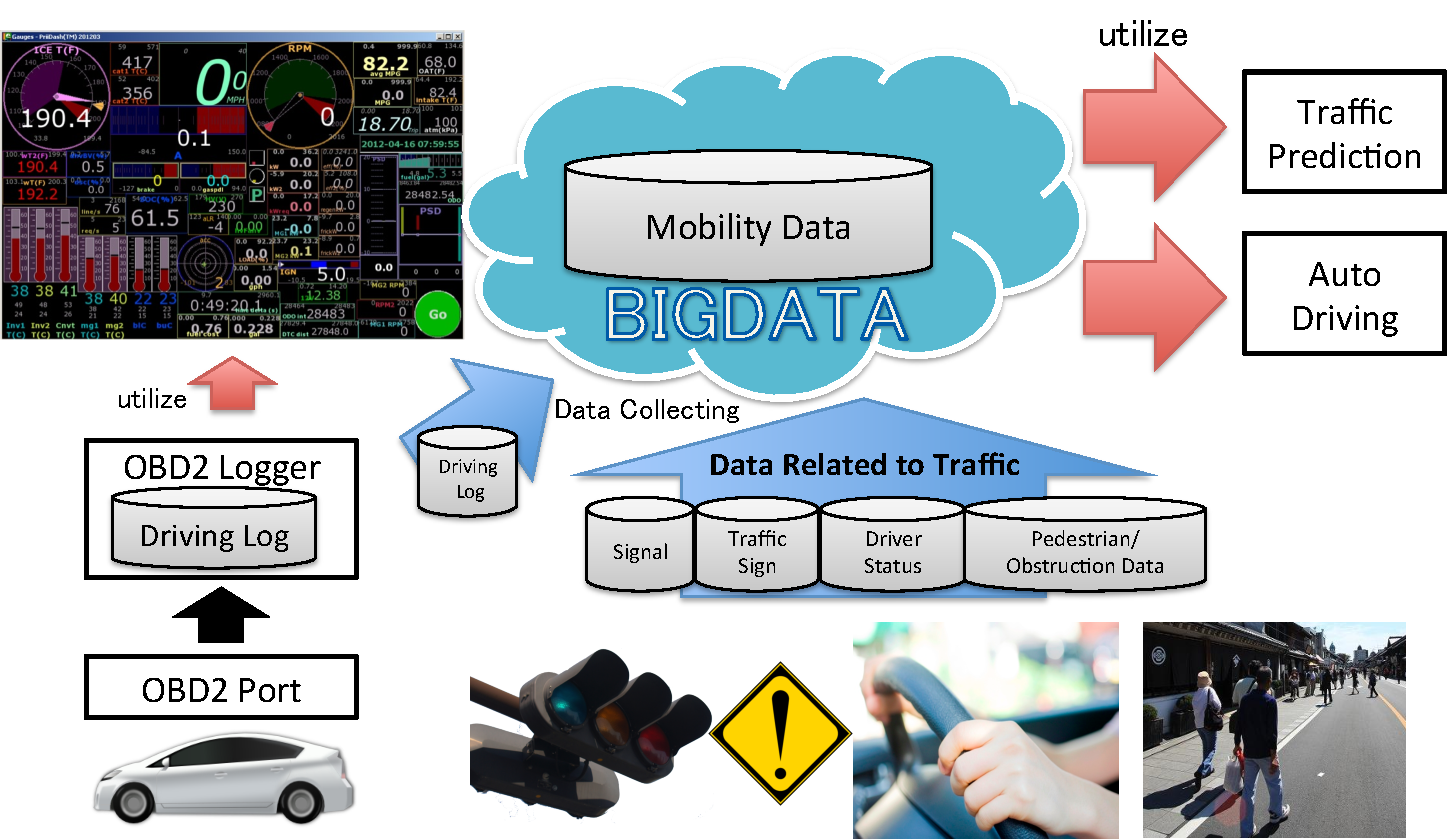
\includegraphics[width=\hsize]{fig/OBD2.pdf}
 \caption{Collecting automotive and environmental data.}
 \label{fig:obd2}
\end{figure}

Fig. \ref{fig:obd2} illustrates an example of collecting automotive data
through the on-board diagnosis (OBD) connectors as well as environmental
data.
We are building this system using commodity ICT products. 
The automotive data can be obtained through the CAN bus, while the
environmental data can be captured using mobile devices such as
smartphones.
These data sets can actually be shared with a lot of mobility CPS
agents.
Such ``Big Data'' trends also encourage the concept of mobility CPS in
the cloud.
Since the data sets are stored in the cloud, each mobility CPS agent
needs to access the network.
For example, we can store a very large global trained data set
\cite{Niknejad12} for anonymous agents to perform image recognition.
The first step towards this approach is to understand the scale of
latency and overhead imposed on cloud computing in real-time.


\section{Prototyping}
\label{sec:prototype}

In this paper, we provide a prototyping of ICT platforms for mobility
CPS applications, particularly taking an example of autonomous driving.
We apply the cloud computing paradigm for autonomous driving to
complement wimpy vehicular embedded systems.
One of the major goals of this cloud-based autonomous driving system is
to offload the computational requirement of autonomic control and
environmental perception to remote HPC servers from local vehicular
systems.
We focus on ICT platforms.
Hence, the implementations of autonomic control and environmental
perception for autonomous driving are outside the scope of this paper.
Interested readers are encouraged to refer to our different
contributions \cite{Hirabayashi13, Kagami13}.

In the rest of this section, we present two ICT platforms for the
development of cloud-based autonomous driving.
The first platform is a smartphone application that controls the vehicle
from remote sources.
The second platform is also a smartphone application that transfers
captured images to the HPC server as fast as possible.

\subsection{Remote Vehicle Control}

\begin{figure}[!t]
 \centering
 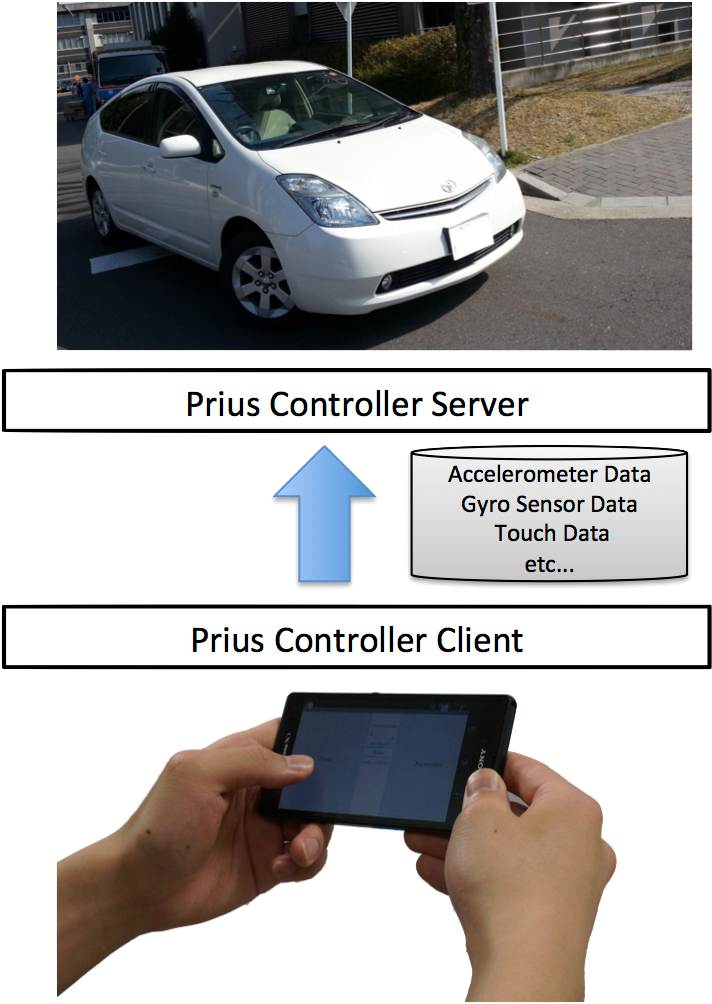
\includegraphics[width=0.6\hsize]{fig/Andrive.pdf}
 \caption{A smartphone application for remote vehicle control.}
 \label{fig:andrive}
\end{figure}

We have a TOYOTA Prius that is modified to be able to overwrite the
control of steering, accelerator, and break from the computer.
This computer called ``vehicular master computer'' is connected to an
supplemental embedded device board that can directly send signals to the
internale wire system controlling the vehicle.
We omit a detailed description of this autonomous driving system, as our
primary focus is the quantification of overhead.

Fig. \ref{fig:andrive} shows a conceptual architecture of our
experimental remote vehicle control system.
We make use of a commodity smartphone to send the control command to the
vehicular master computer equipped within the vehicle through the network.
The smartphone application determines the steering angle from the gyro
sensor while the accelerator and the break strokes are controlled by the
graphics user interface.
Thus, we can intuitively use a smartphone as if it were a game
controller of the vehicle remotely.

\subsection{Networked Image Processing}

\begin{figure}[!t]
 \centering
 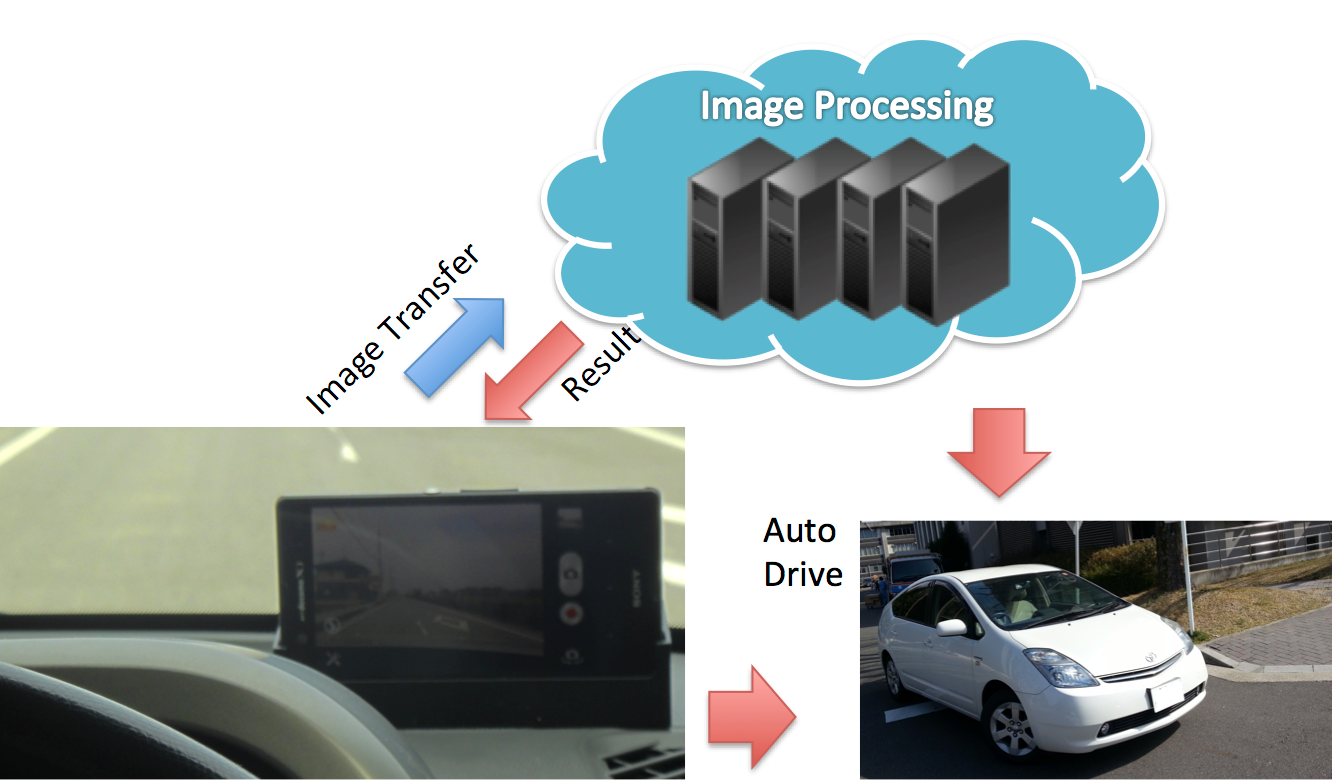
\includegraphics[width=0.9\hsize]{fig/TIPIC.pdf}
 \caption{Networked image processing.}
 \label{fig:tipic}
\end{figure}

Environmental perception is composed of compute-intensive tasks.
Perception algorithms are often complex and the volume of input data
from laser sensors and high-resolution cameras is not afforable for
mobile embedded systems.
Therefore it is significant if we can offload these compute-intensive
tasks to the cloud in real-time.

Fig. \ref{fig:tipic} shows a conceptual architecture of our experimental
networked image processing system.
We capture images in real-time from commodity smartphones attached in
the vehicle and transfer them over the network to the HPC server where
the actual image processing tasks are executing.
The results of image processing such as the detected vehicles and
pedestrians are fed back to the vehicular embedded system.
Although we have implemented several variants of state-of-the-art image
processing algorithms \cite{Hirabayashi13}, we exclude them from the
scope of this paper.
Alternatively we investigate if commodity ICT platforms can meet the
requirement of throughput and latency for image transfers.

Unlike control commands, the size of an image is large and it generates
additional latency for the transfer.
For example, each image transfer is composed of (i) capturing an image,
(ii) encoding that image, and (iii) transferring the encoded image.
Since these three stages can be pipelined, the total throughput would
benefit from multithreading and a multicore processor.
Furthermore, we have observed that the encoding stage is much longer
than the capture and the transfer stages when we use a smartphone as a
client due to its wimpy embedded processor performance.
This means that the effective rate of image capture and transfer may be
limitted to the execution time of encodling.
In order to maximize the image transfer throughput on an embedded
multicore processor, we increase the number of threads for encoding as
shown in Fig. \ref{fig:multithread}.
In this example, one can see that the second (blue) transfer does not
have to stall before the encoding stage because another thread is
available for encoding whereas it would stall due to the preceding
encoding process if there is only one thread available for encoding.
Thus, we suggest that networked image processing using smartphones
should make use of the multithreading capability and the parallelism of
embedded multicore processors.

\begin{figure}[!t]
 \centering
 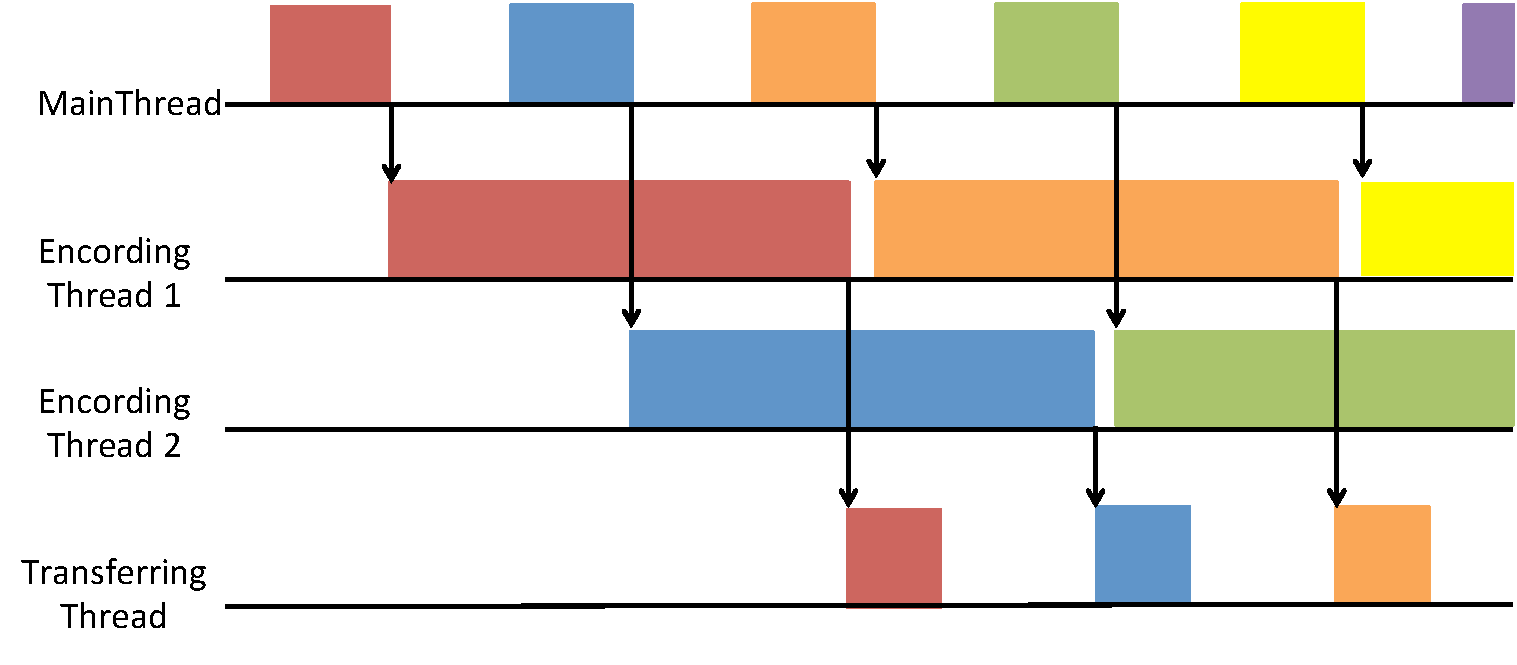
\includegraphics[width=0.9\hsize]{fig/multithread.pdf}
 \caption{Multithreading of image transfers.}
 \label{fig:multithread}
\end{figure}


\section{Evaluation}
\label{sec:evaluation}

We now evaluate the data transfer overhead in the context of cloud-based
autonomous driving.
We assume that autonomic control and environmental perception are
provided in the remote server, but they are not within the scope of this
paper.
What we focus on in this experiment is the measurement of the data
transfer overhead.

\subsection{Control Command Transfer}

This experiment measures the transfer time taken to send control
commands to the vehicle from a smartphone.
The commands control the steering, accel, and brake of the vehicle.
The steering angle is determined by the gyro sensor data while the accel
and break strokes are manipulated by the graphics user interface of the
Andrive application.
We use the HTC J butterfly Snapdragon S4 Pro (APQ8064@1.5GHz, Quad Core)
for a testing smartphone.

\begin{figure}[!t]
 \centering
 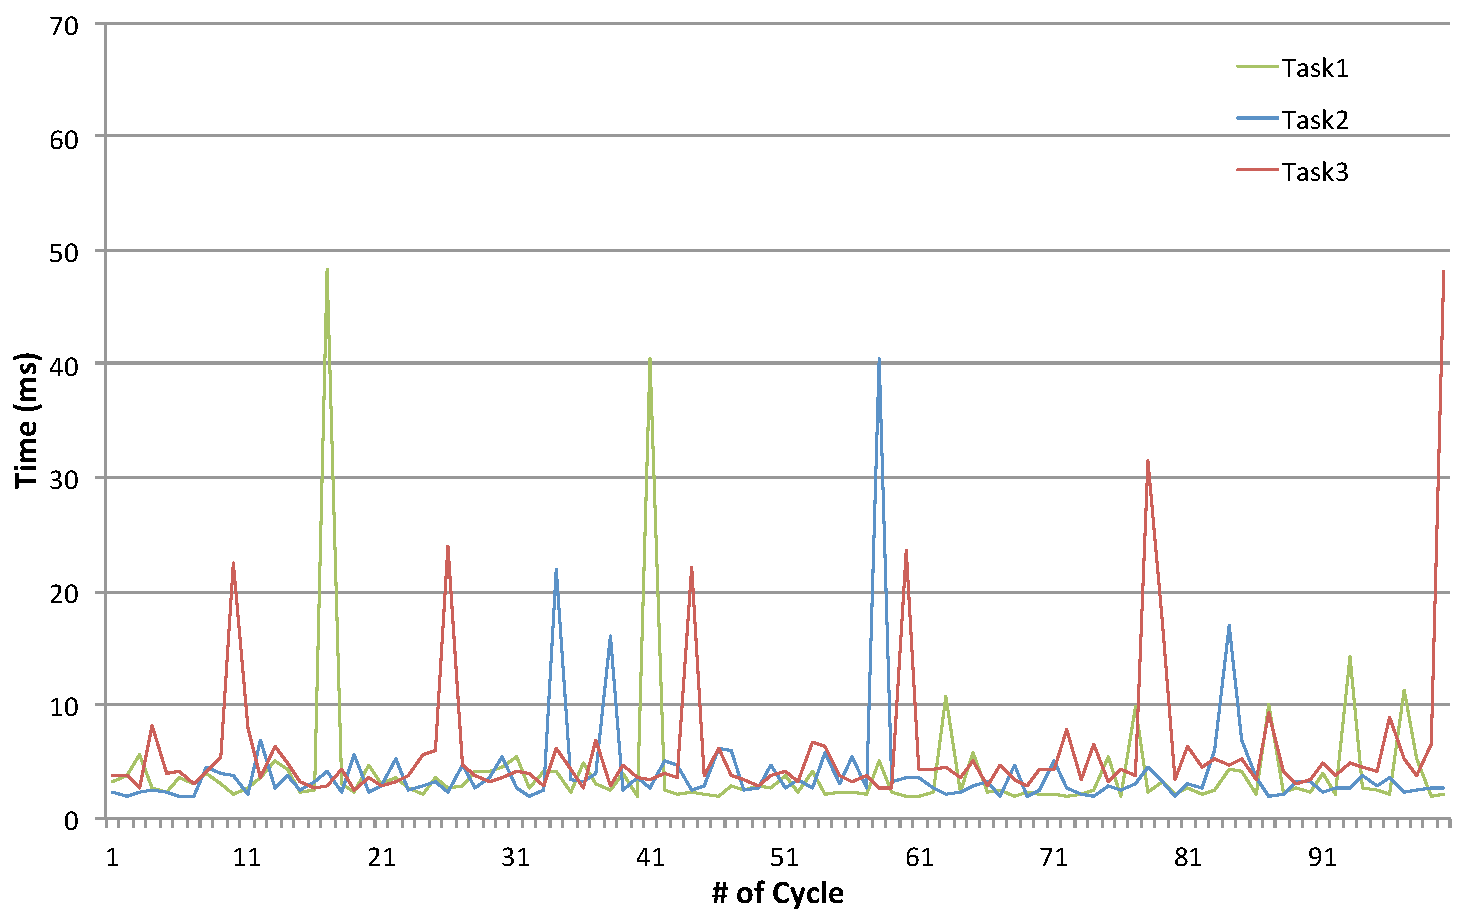
\includegraphics[width=\hsize]{fig/No1_Andrive_serv_cycle_WiFi.pdf}
 \caption{The synchronous transfer time for control commands using WiFi.}
 \label{fig:no1}
\end{figure}

Fig. \ref{fig:no1} shows the transfer time for control commands using
WiFi.
Note that the PC server sends back an acknowledge message to the
smartphone client every time the commands are received.

\begin{figure}[!t]
 \centering
 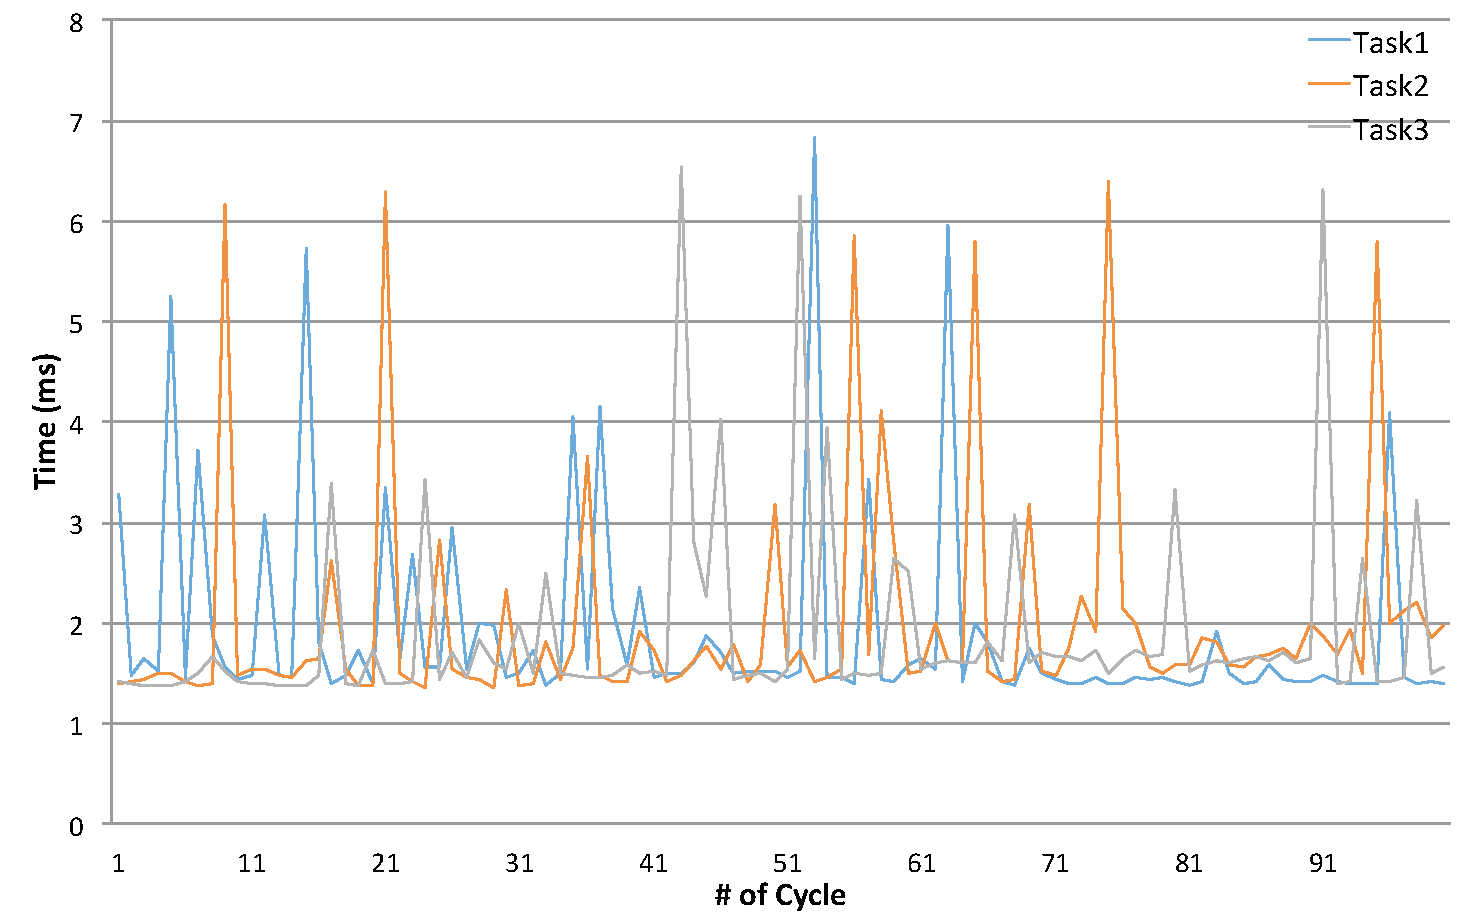
\includegraphics[width=\hsize]{fig/No4_Andrive_serv_cycle_WiFi_only_send.pdf}
 \caption{The asynchronous transfer time for control commands using WiFi.}
 \label{fig:no4}
\end{figure}

\begin{figure}[!t]
 \centering
 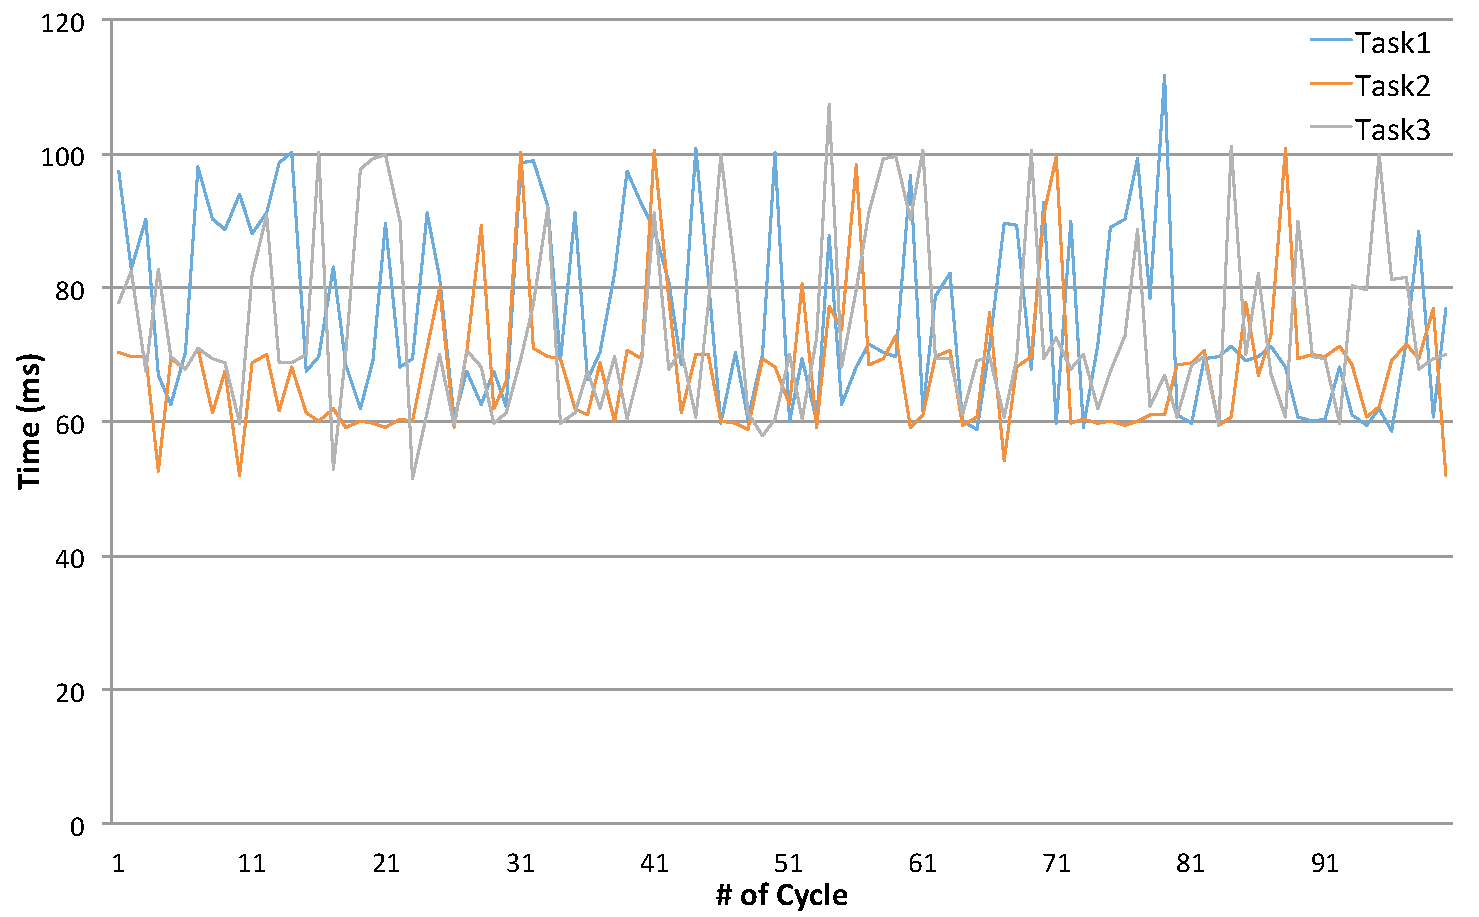
\includegraphics[width=\hsize]{fig/No2_Andrive_serv_cycle_LTE.pdf}
 \caption{The synchronous transfer time for control commands using LTE.}
 \label{fig:no2}
\end{figure}

\begin{figure}[!t]
 \centering
 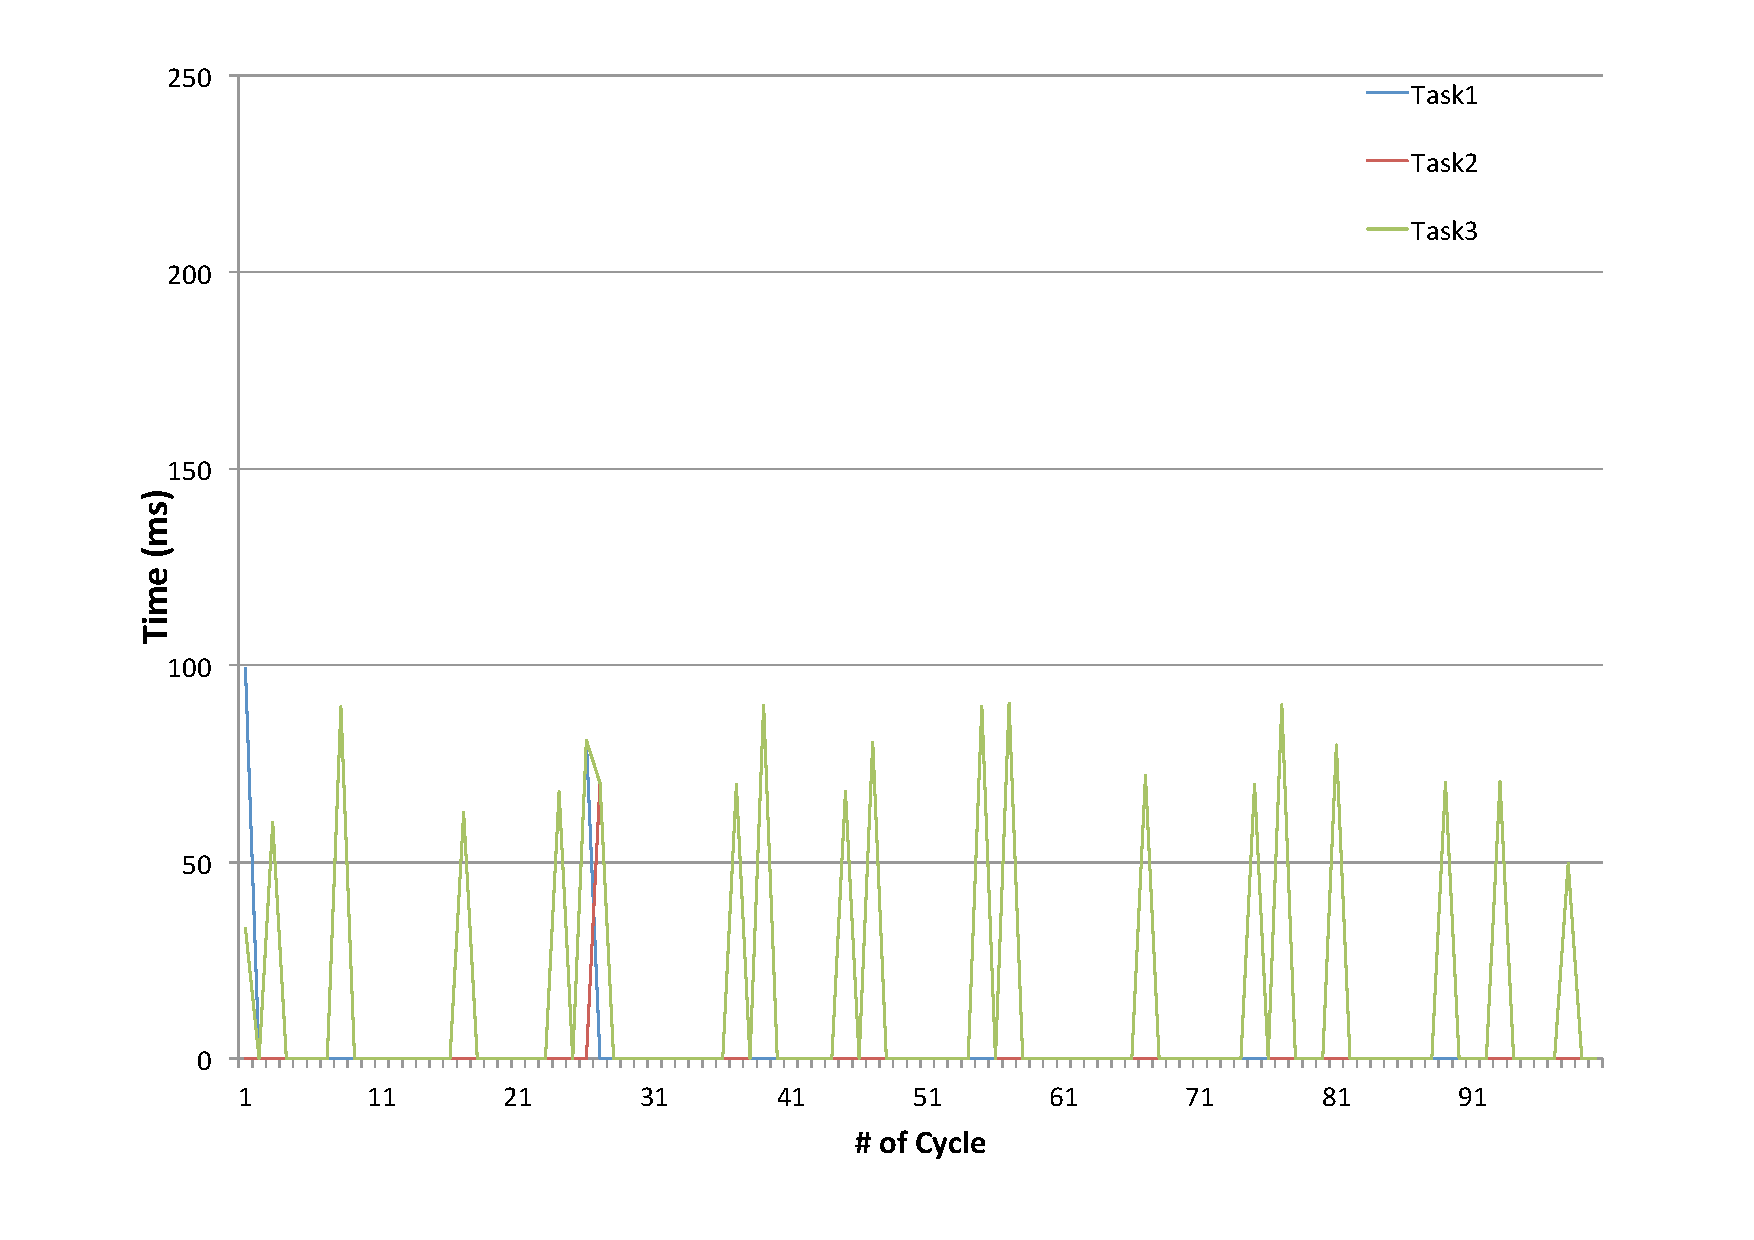
\includegraphics[width=\hsize]{fig/No5_Andrive_serv_cycle_LTE_only_send.pdf}
 \caption{The asynchronous transfer time for control commands using LTE.}
 \label{fig:no5}
\end{figure}

\begin{figure}[!t]
 \centering
 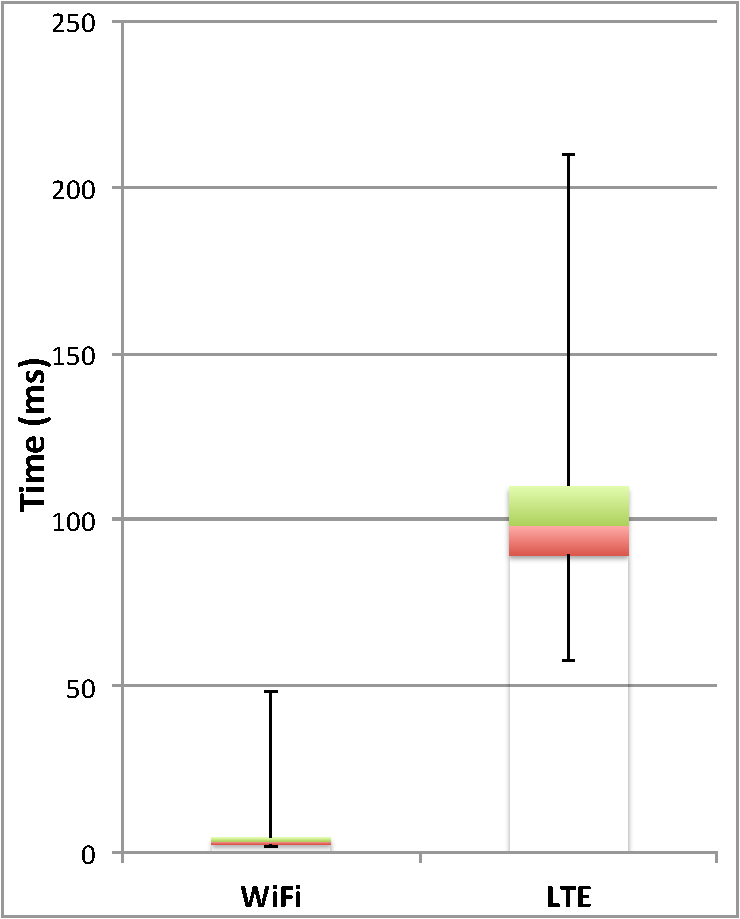
\includegraphics[width=0.45\hsize]{fig/No3_Andrive_boxplot_compare_WiFi_and_LTE.pdf}
 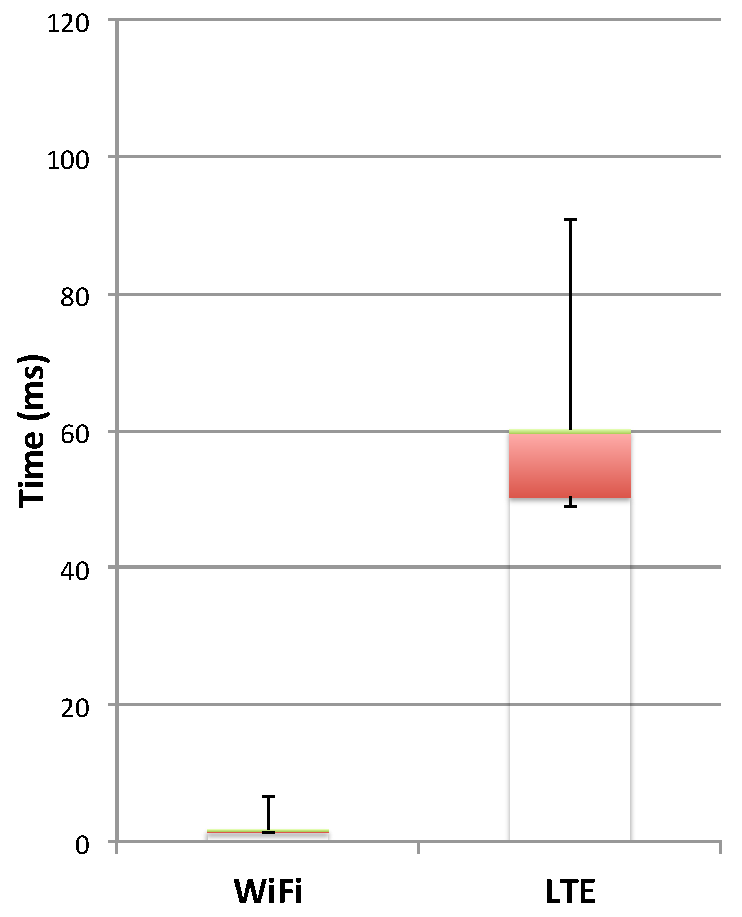
\includegraphics[width=0.45\hsize]{fig/No7_Andrive_only_send_boxplot_compare_WiFi_and_LTE.pdf}
 \caption{Summarized box plotting of the transfer times.}
 \label{fig:no3_7}
\end{figure}

\begin{figure}[!t]
 \centering
 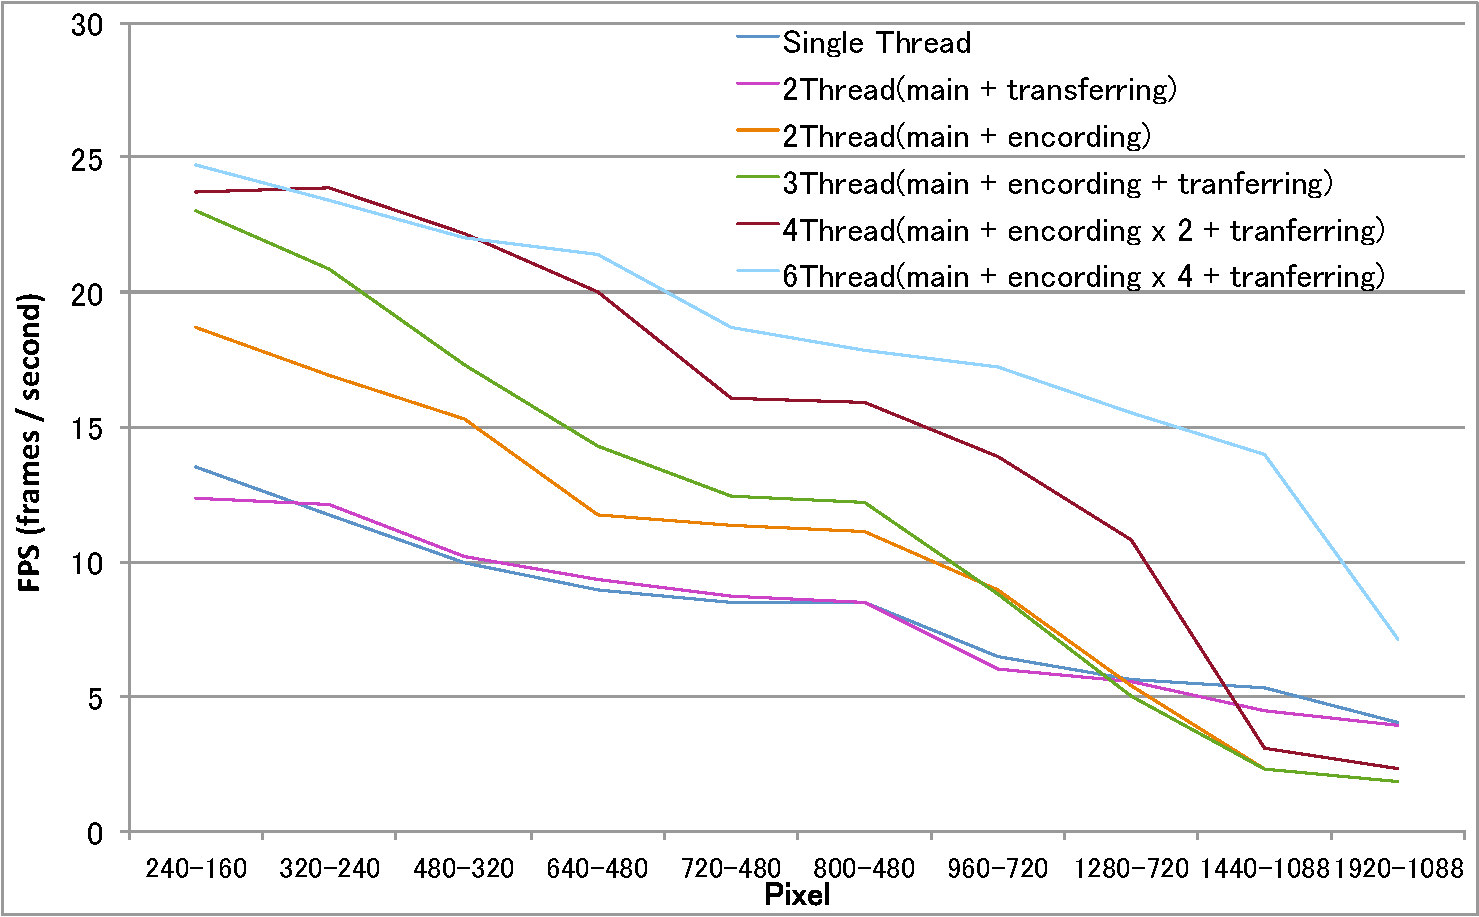
\includegraphics[width=\hsize]{fig/No8_TIPiC_FPS_graph_WiFi.pdf}
 \caption{The frame rate of networked image processing using WiFi.}
 \label{fig:no8}
\end{figure}

\begin{figure}[!t]
 \centering
 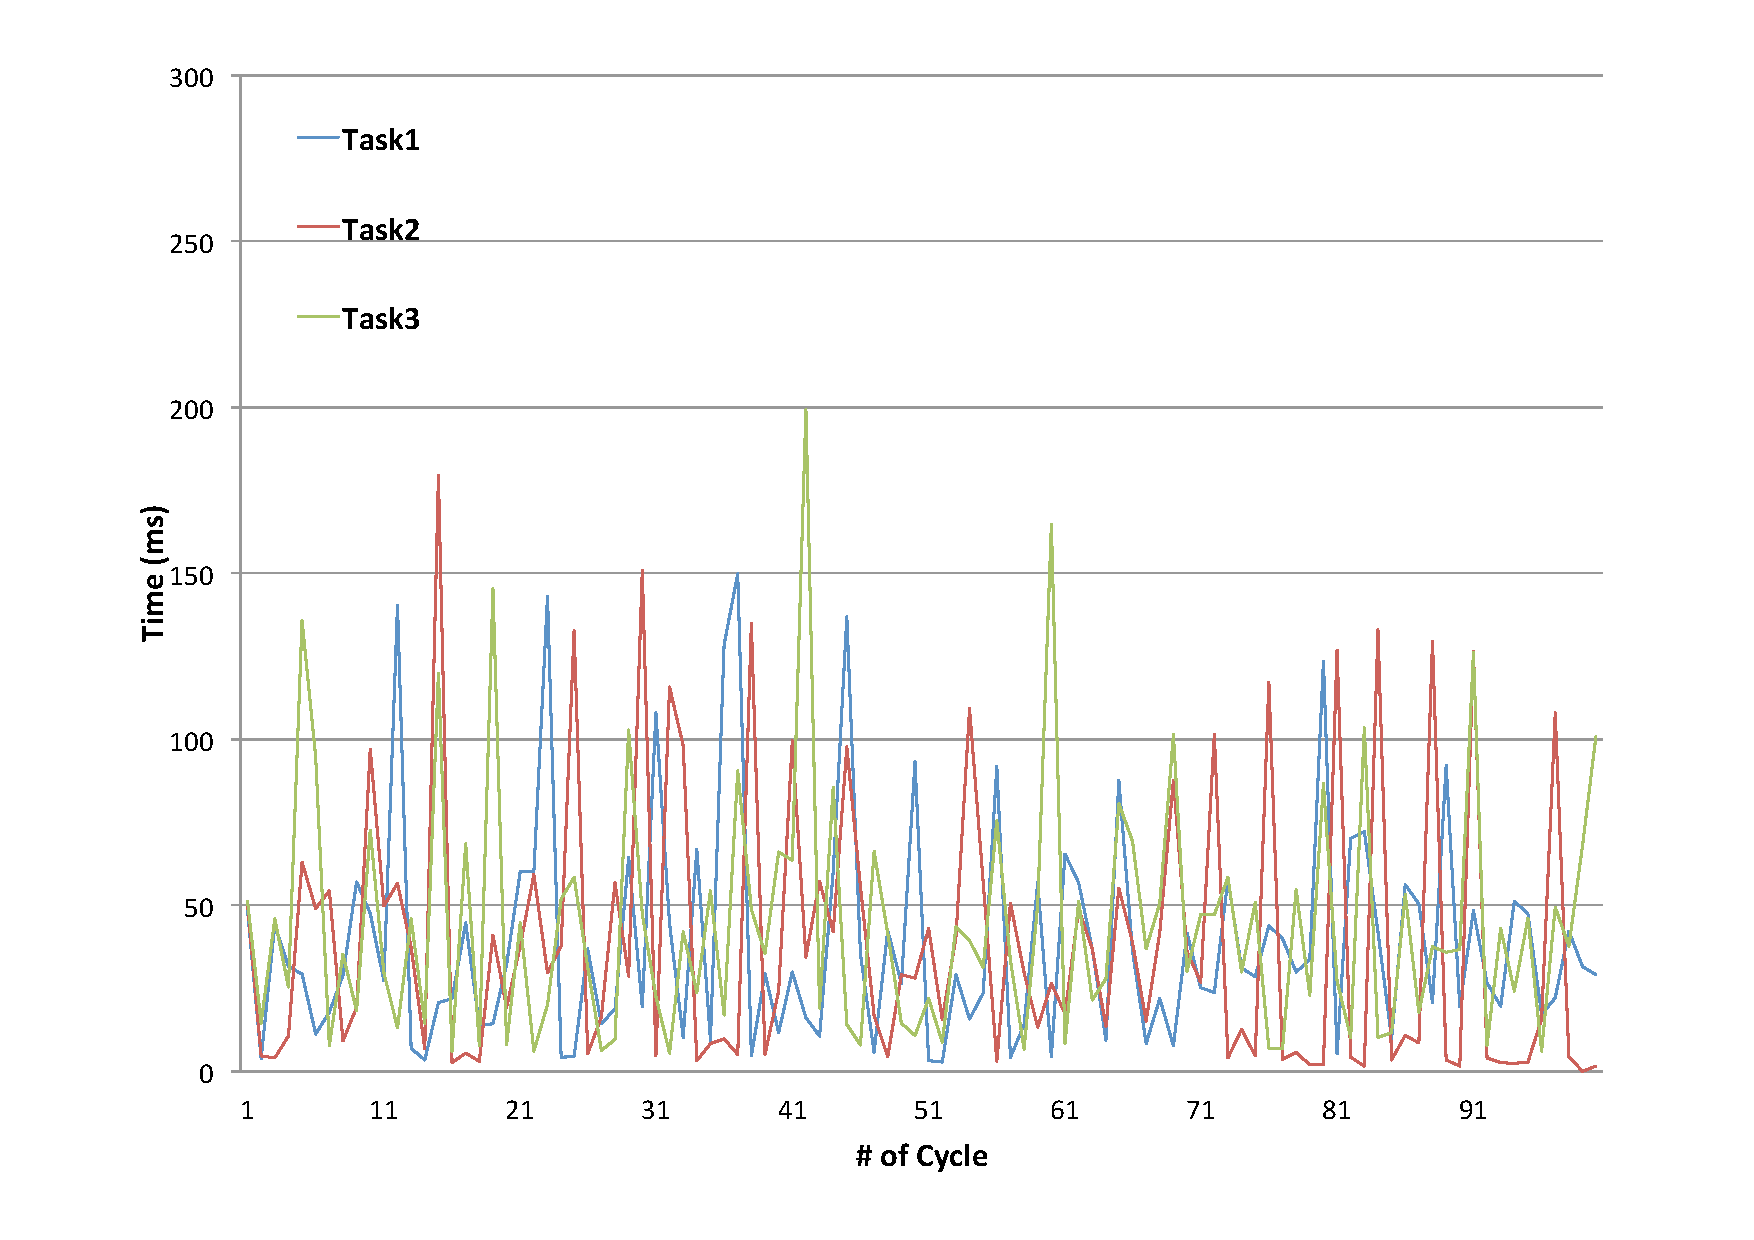
\includegraphics[width=\hsize]{fig/No9_TIPiC_serv_cycle_WiFi.pdf}
 \caption{The arrival time of networked image processing using WiFi.}
 \label{fig:no9}
\end{figure}

\begin{figure}[!t]
 \centering
 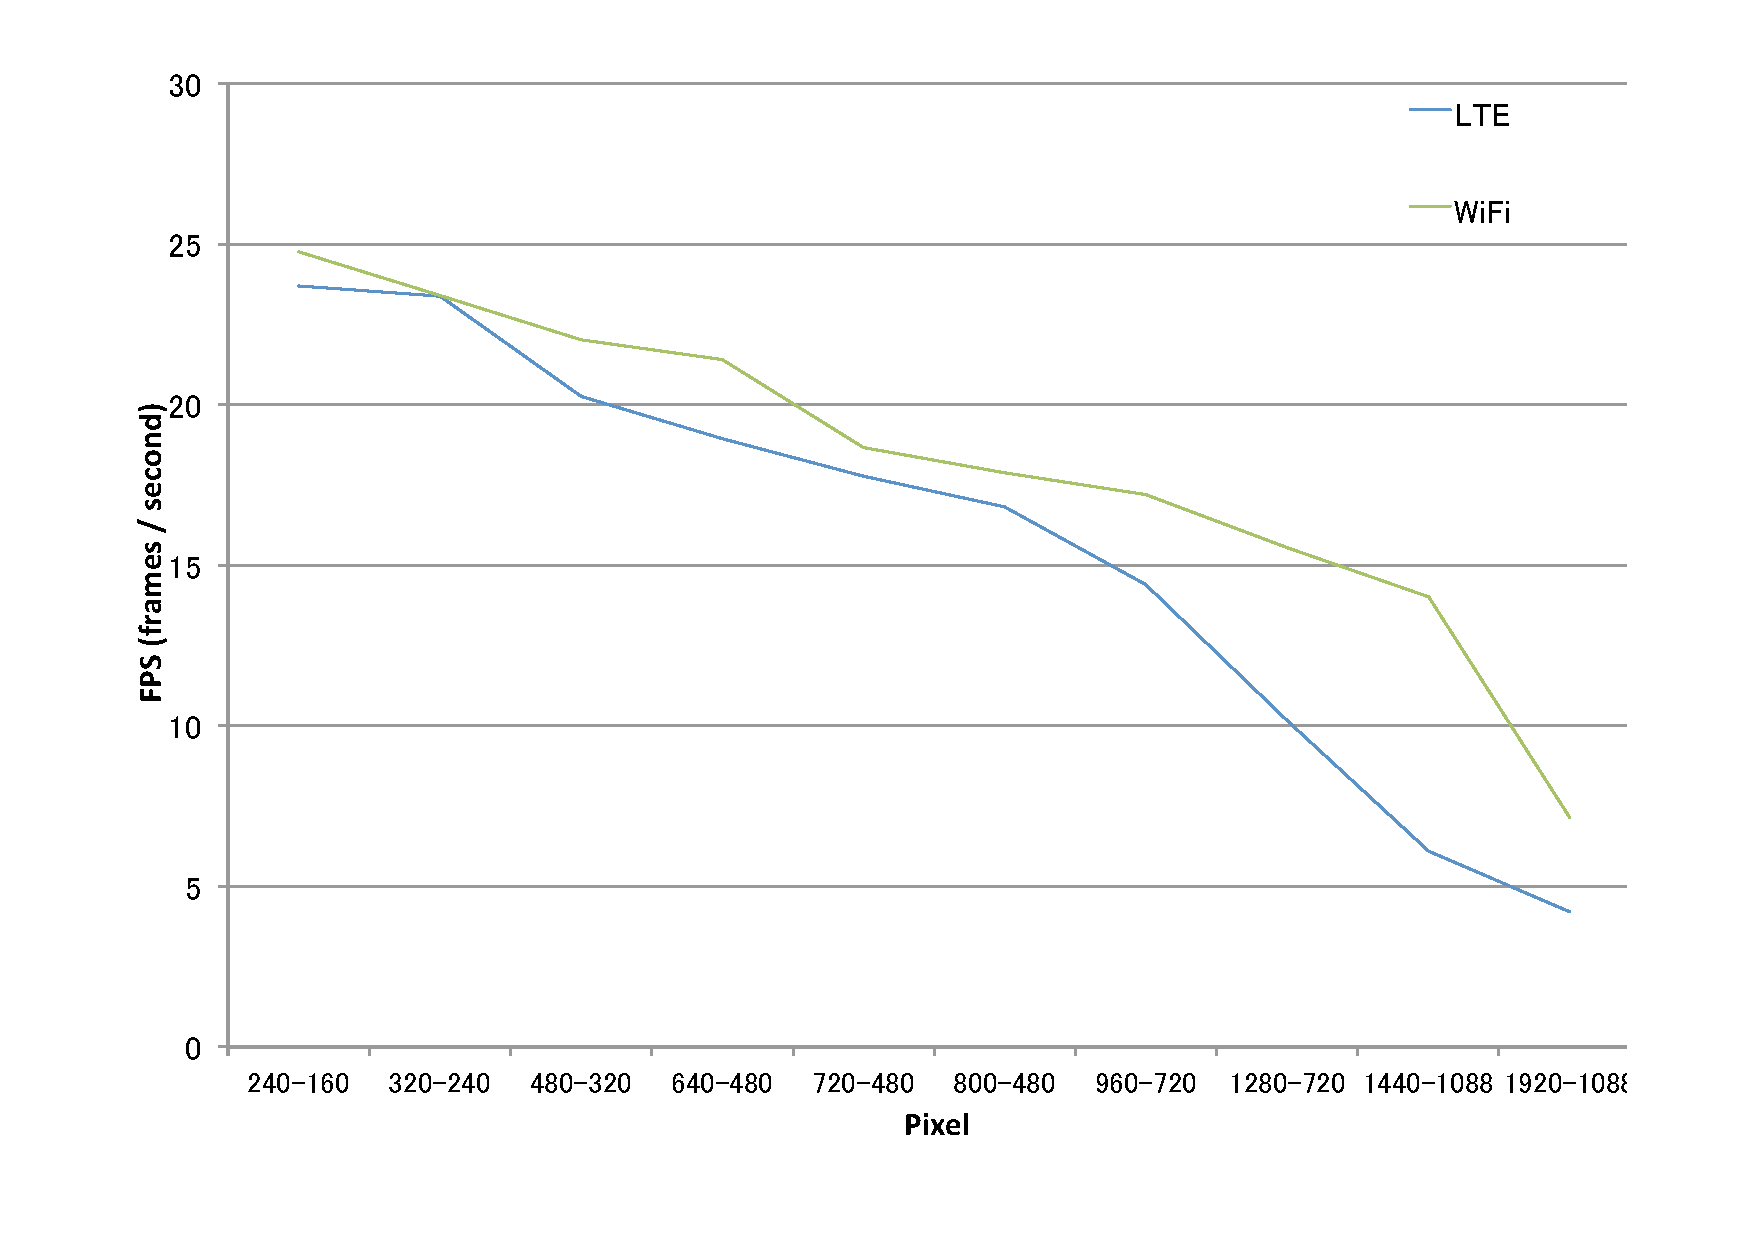
\includegraphics[width=\hsize]{fig/No10_TIPiC_FPS_graph_LTE.pdf}
 \caption{The frame rate of networked image processing using LTE.}
 \label{fig:no10}
\end{figure}

\begin{figure}[!t]
 \centering
 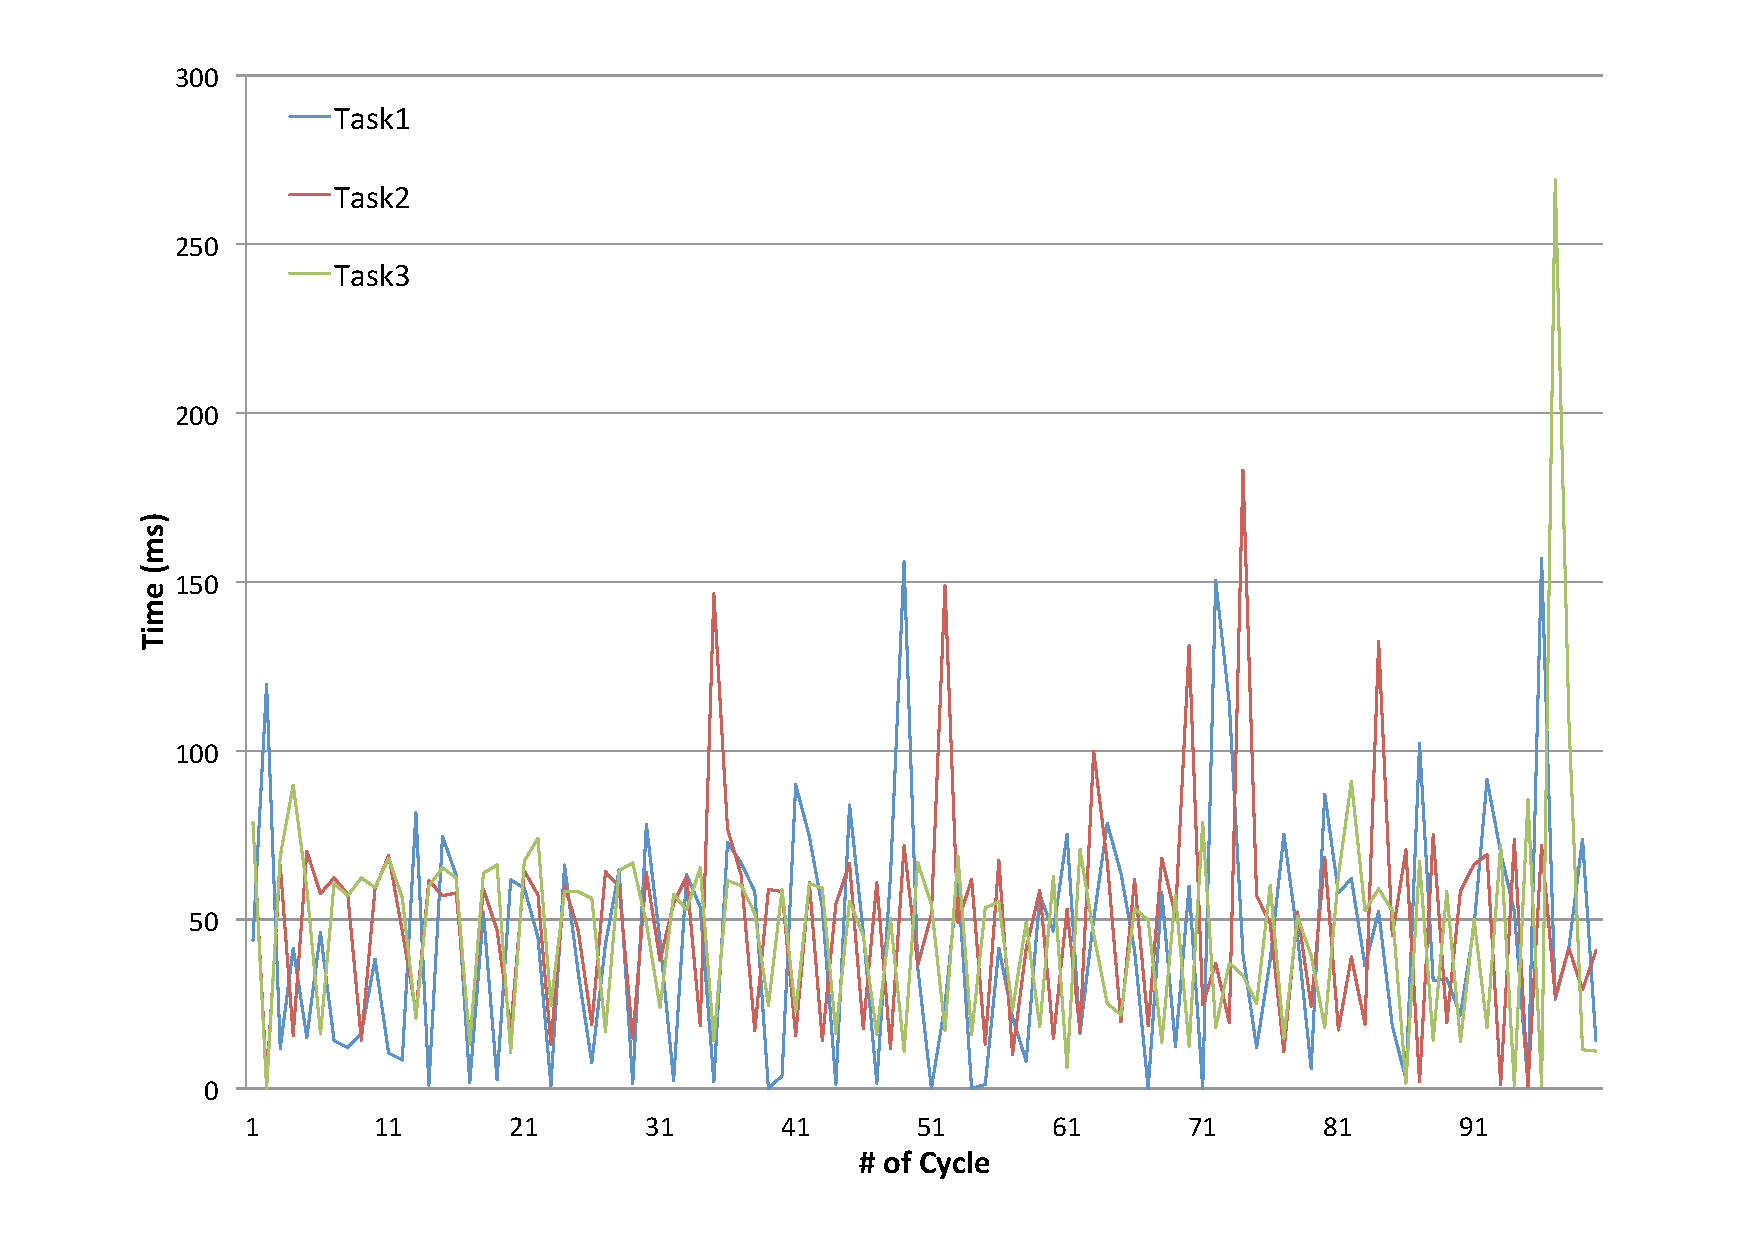
\includegraphics[width=\hsize]{fig/No11_TIPiC_serv_cycle_LTE.pdf}
 \caption{The arrival time of networked image processing using LTE.}
 \label{fig:no11}
\end{figure}

\begin{figure}[!t]
 \centering
 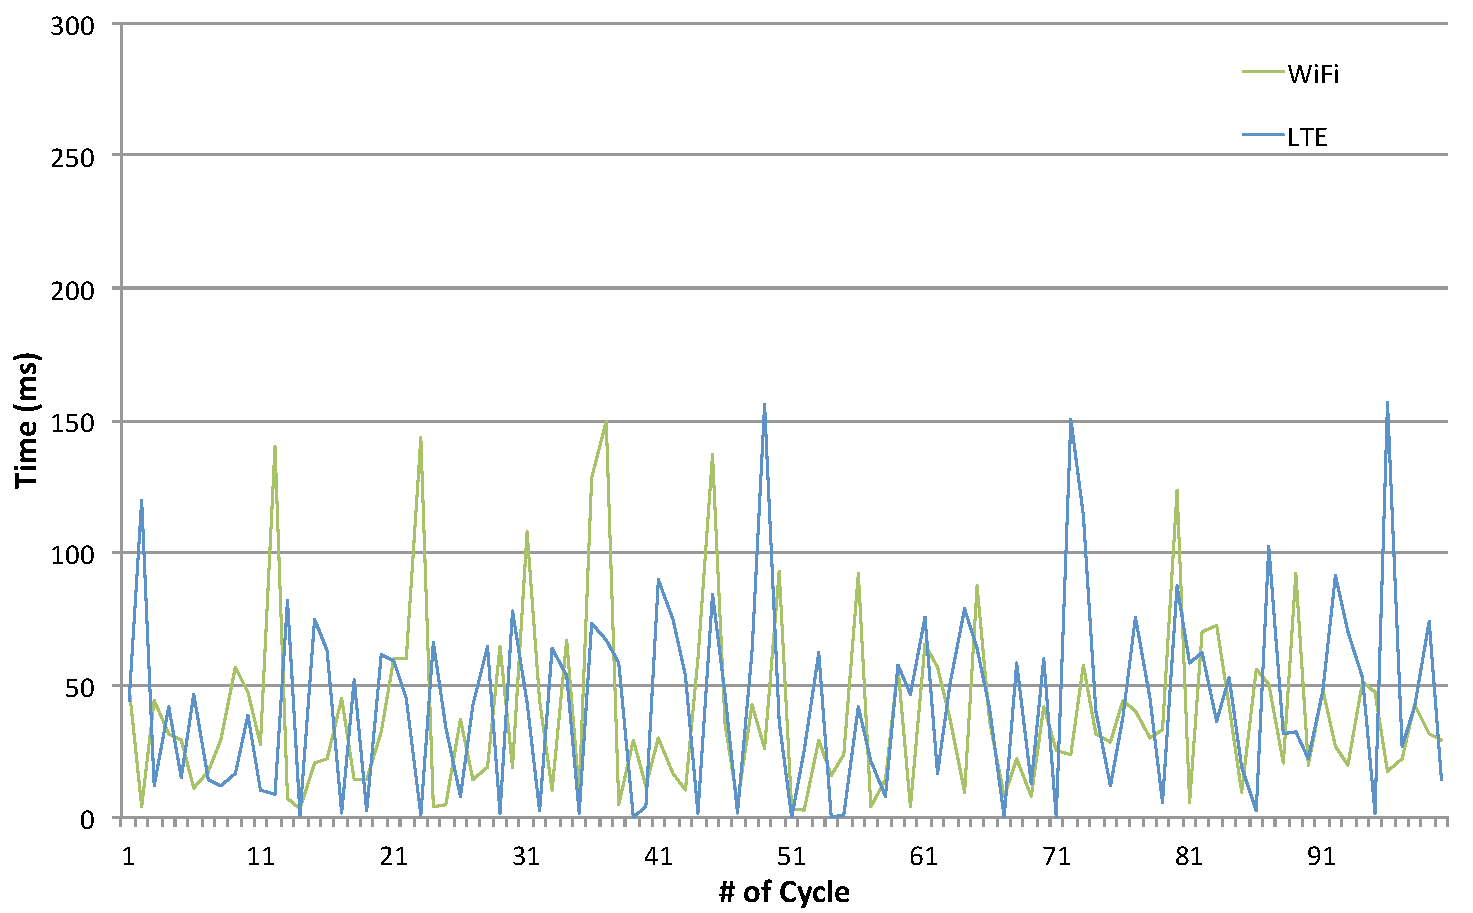
\includegraphics[width=\hsize]{fig/No12_TIPiC_serv_cycle_compare_WiFi_and_LTE.pdf}
 \caption{A comparison of the arrival times.}
 \label{fig:no12}
\end{figure}

\begin{figure}[!t]
 \centering
 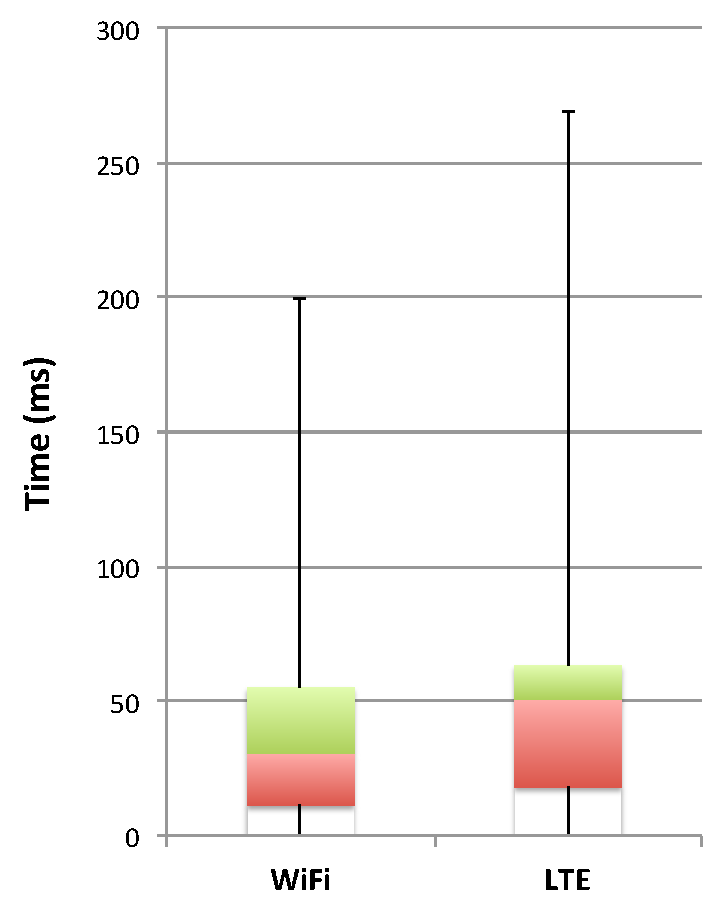
\includegraphics[width=0.5\hsize]{fig/No13_TIPiC_boxplot_compare_WiFi_and_LTE.pdf}
 \caption{Summarized box plotting of the arrival times.}
 \label{fig:no13}
\end{figure}

\begin{figure}[!t]
 \centering
 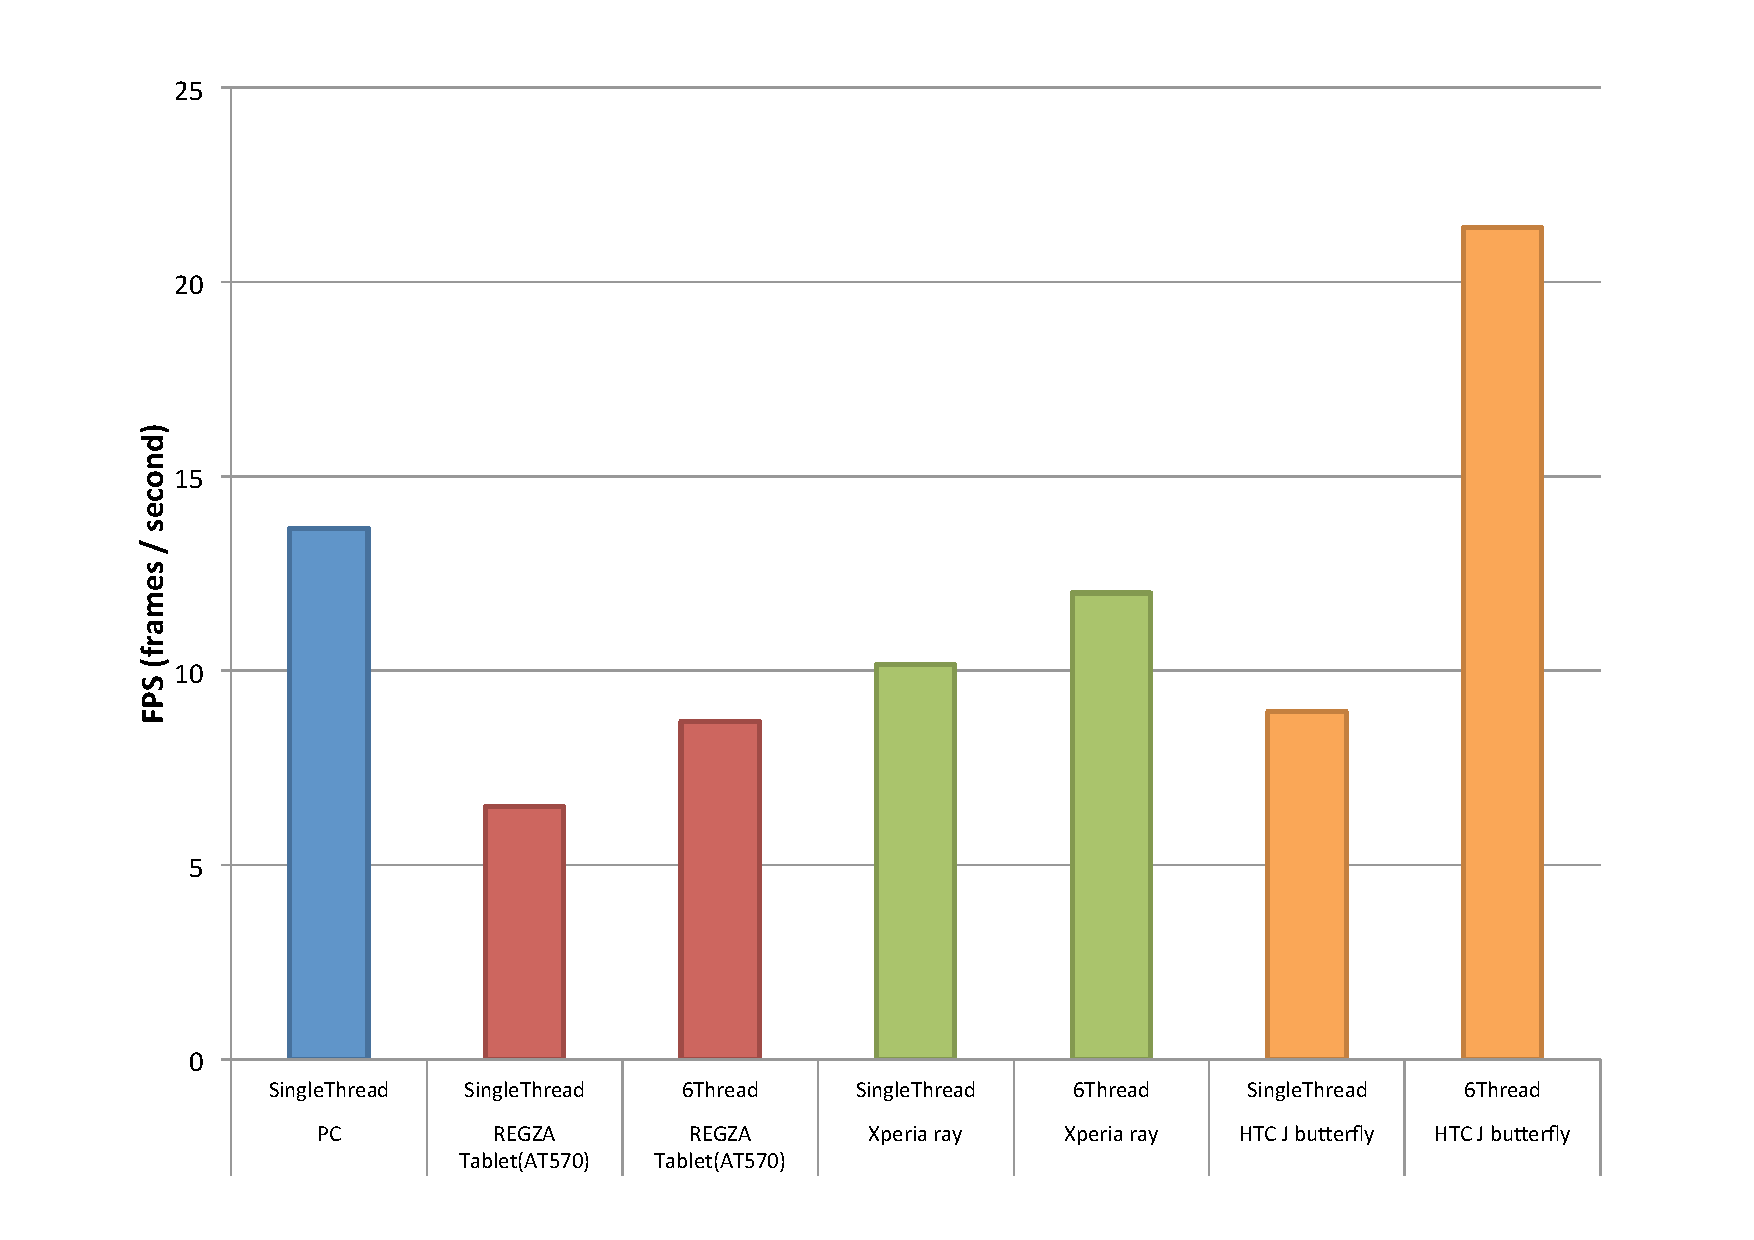
\includegraphics[width=\hsize]{fig/No14_Android_and_PC_benchmarck.pdf}
 \caption{Performance differences of a smartphone and PC.}
 \label{fig:no14}
\end{figure}

\section{Conclusion}
\label{sec:conclusion}

In this paper, we have presented GPU implementations of HOG-based object
detection and their performance evaluation.
Unlike preceding work that highly stressed on performance improvements,
our implementations are based on an analysis of performance bottlenecks
posed due to an introduction of the deformable models in HOG-based
object detection.
This approach ensures that the GPU truly accelerates approapriate
computational blocks.
Our evaluation using a commodity GPU showed that our GPU implementation
can speed up the existing HOG-based vehicle detection program tailored
to the deformable models by 1.5x to 3x over traditional CPU
implementations.
Given that this performance improvement is obtained from the entire
program runtime rather than particular algorithm parts of the program,
our contribution is useful and significant for real-world applications
of vision-based object detection. 

To the best of our knowledge, this is the first piece of work that made
a \textit{tight} coordination of object detection and parallel computing
-- a core challenge of CPS.
Specifically we showed that a measured and structured way of GPU
programming is efficient for the object detection program and quantified
the impact of GPUs in performance.
Our conclusion is that GPUs are promising to meet the required
performance of vision-based object detection in the real world.

In future work, we plan to complement this work with systemized
coordinations of computations and I/O devices.
Since real-world applications require camera sensors to obtain input
images while GPUs are compute devices off the host computer, the data
I/O latency could become a non-trivial bottleneck on the data bus.
In this scenario, we need enhanced system support such as zero-copy
approaches \cite{Kato13} to minimize the data latency raised between
camera sensors and GPUs.
We also plan to augment our GPU implementations using multiple GPUs in
order to meet the real-time and real-fast requirement of real-world CPS
applications.


\bibliographystyle{plain}
{\footnotesize
\bibliography{references}
}

\end{document}



